\documentclass{beamer} % if hadout \documentclass[12pt, handout]{beamer}
\usepackage[utf8]{inputenc}
\usepackage[frenchb,noconfigs]{babel}
\usepackage{lmodern,textcomp,ifthen,graphicx,enumitem,booktabs,csvsimple}
\usepackage{beamerx}

%% Tamaño figuras
\newlength{\mylength}
\setlength{\mylength}{0.47\textwidth}

\begin{document}
	
	%%% - Titulo del beamer %%
	\title[Felipe García]{Modal SNA  \\ Sûreté aérienne}[Sûreté\\ aérienne]
	\author[]{Felipe García}
		
	\maketitle
	%--- Next Frame ---%
	
	\begin{frame}[t]{Plan}
		\tableofcontents
	\end{frame}
	%--- Next Frame ---%
	
	\section{Introduction} % (fold)
	\label{sec:introduction}
	
	
	\begin{frame}[t]{Collision entre Avions}
		Faits autour des avions : 
		\begin{itemize}
			\item<+-> 80.000 vols par jour
			\item<+-> Plusieurs risques
			\item<+-> Collision entre Avions
		\end{itemize}
		
		\only<1>{\begin{figure}[htbp]
			\centering
			\begin{minipage}[b]{0.5\textwidth}
				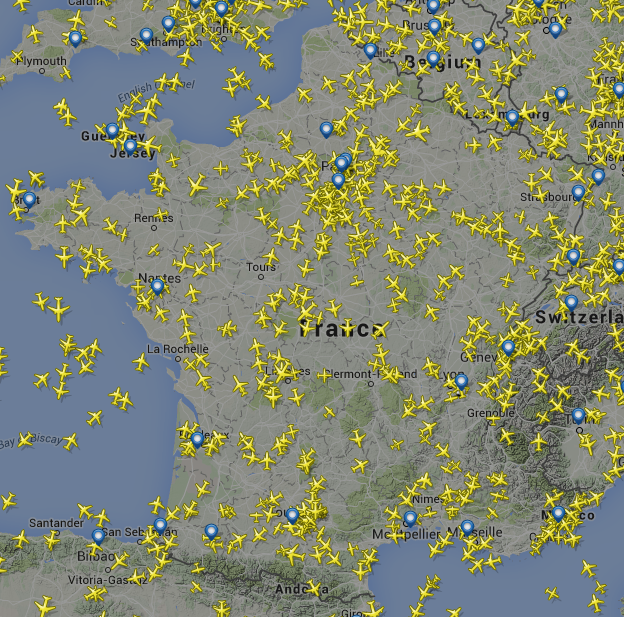
\includegraphics[width=\textwidth]{Images/VolsFrance}
			%\caption{Vols en temps réel}
			\label{fig:Vols}
			\end{minipage}
		\end{figure}}
		
		
	\end{frame}
	% section introduction (end)
	
	\subsection{Modélisation} % (fold)
	\label{subsec:modelisation}
	
	\begin{frame}[t]{Routes des Avions}
		\begin{itemize}
			\item<+-> Route divisé en waypoints
			\item<+-> Composante aléatoire : le vent
			\item<+-> Processus stochastique $X_t=(X_{a,t},X_{c,t})$
			\begin{align*}
				\mathrm d X_t &= v ~ \mathrm d t+\sigma_t ~ \mathrm d W_t
			\end{align*}
			
		\end{itemize}
	\end{frame}
	%--- Next Frame ---%
	\begin{frame}[t]{Modélisation Aléatoire}
		\begin{itemize}
			\item<+->  Modélisation aléatoire 
			\begin{align*}
				\mathbb{C}\mathrm{ov}(X_{a,t},X_{a,s}) &= r_a^2 t^2 \\
				\mathbb{C}\mathrm{ov}(X_{c,t},X_{c,s}) &= \sigma_{c}^2 (1-e^{-2\frac{r_c}{\sigma_c}v(s-t)})e^{-\frac{r_c}{\sigma_c}v(s-t)}
			\end{align*}
			\item<+-> Connu comme processus d'Ornstein-Uhlenbeck
			\item<+-> Le processus reste gaussien avec une rotation
			
		\end{itemize}
	\end{frame}
	%--- Next Frame ---%
	% section modelisation (end)
	
	\subsection{Simulation} % (fold)
	\label{subsec:simulation}
	
	\begin{frame}[t]{Modélisation des trajectoires}
		Méthode de modélisation.
		\begin{itemize}
			\item<+-> Trajectoires discrétisées
			\item<+-> On simule la différence des trajectoires $U=X^{(1)} - X^{(2)}$
			\item<+-> On modélise des trajectoires en parallèle et croisées
		\end{itemize}
	\end{frame}
	%--- Next Frame ---%
	\begin{frame}[t]{Probabilité de Collision}
		Estimer la probabilité de que la distance entre les avions soit inférieure à un seuil prédéfini $\epsilon$.
		\begin{subequations}
		\begin{align*}
			\mathbb{P}\left(\exists i~|~ \lVert X^{(1)}_{i} - X^{(2)}_{i} \rVert_2 \leq \epsilon \right)
			&= \mathbb{P}\left(\bigcup_{i=1}^{d} \lVert X^{(1)}_{i} - X^{(2)}_{i} \rVert_2 \leq \epsilon  \right)  \\
			&= \mathbb{P}\left(\min_{1\leq i\leq d} \lVert X^{(1)}_{i} - X^{(2)}_{i} \rVert_2 \leq \epsilon \right)  \\
			&= 1-\mathbb{P}\left(\forall i~|~ \lVert X^{(1)}_{i} - X^{(2)}_{i} \rVert_2 \leq \epsilon \right) \label{eq:numerique}
		\end{align*}
		\end{subequations}
	\end{frame}
	%--- Next Frame ---%
	% section simulation (end)
	
	\section{Résultats} % (fold)
	\label{sec:resultats}
	
	\begin{frame}[t]{Estimation des probabilités}
		\begin{itemize}
			\item<+-> Estimation avec les méthodes du cours
			\item<+-> Vérification des résultats avec une méthode numérique 
			\item<+-> Exemple de trajectoire 
		\end{itemize}
		\only<3>{\begin{figure}[htbp]
					\begin{minipage}[b]{0.8\textwidth}
							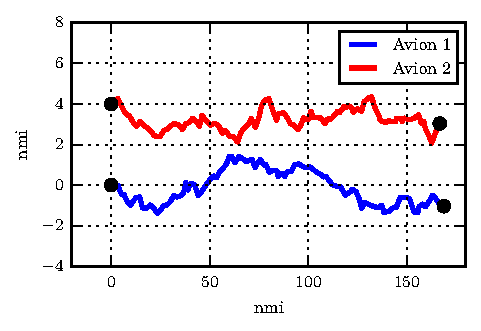
\includegraphics[width=\textwidth]{Images/Script_5_1}
							%\caption{Exemple de Trajectoire}
							\label{fig:trajtype}
						\end{minipage}
					\end{figure}}
	\end{frame}
	
	%--- Next Frame ---%
	\subsection{Monte Carlo naïve} % (fold)
	\label{sub:monte_carlo_naive}
	
	\begin{frame}[t]{Monte Carlo naïve}
		Estimation de $\mathbb{E}[\phi(U)]$ avec $\phi(U)=\mathbb{I}\left \{\min_{1\leq i \leq d} U_i \leq \epsilon \right \}$ et $U=X^{(1)} - X^{(2)}$.
		\only<2>{\begin{table}[htbp]
			\begin{center}
				\csvautobooktabular{Tables/MonteCarlo.csv}
			\end{center}
			%\caption{Estimation avec Monte Carlo de la probabilité de collision}
			\label{tab:MC}
		\end{table}}
		
	\end{frame}
	%--- Next Frame ---%
	\begin{frame}[t]{Distribution Conditionnelle}
		\only<1>{\begin{figure}[htbp]
			\centering
			\begin{minipage}[b]{0.9\textwidth}
				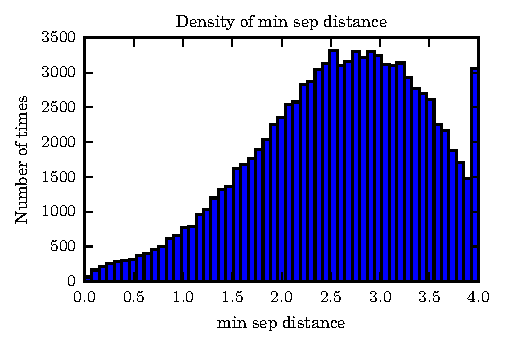
\includegraphics[width=\textwidth]{Images/Script_5_4}
				%\caption{Histogramme de la distance minimale}
				\label{fig:MChist1}
			\end{minipage}
		\end{figure}}
		\only<2>{\begin{figure}[htbp]
			\centering
				\begin{minipage}[b]{0.9\textwidth}
					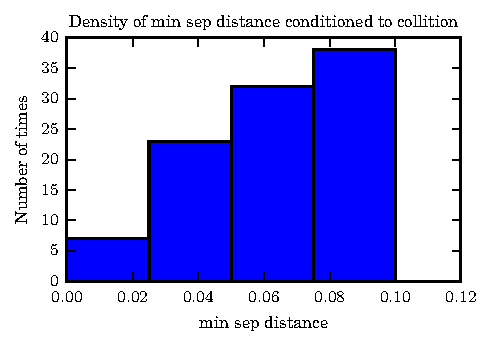
\includegraphics[width=\textwidth]{Images/Script_5_3}
					%\caption{Histogramme de la distance minimale conditionné à la collision}
					\label{fig:MChist2}
				\end{minipage}
			\label{fig:label}
		\end{figure}}
	\end{frame}
	%--- Next Frame ---%
	% subsection monte_carlo_naive (end)
	
	\subsection{Importance Sampling} % (fold)
	\label{sub:importance_sampling}
	
	\begin{frame}[t]{Importance Sampling}
		Implémentation du décentrage.
		\begin{itemize}
			\item<+-> Faire un décentrage adapté au processus
			\begin{align*}
				\mathbb{E}(f(\boldsymbol x)) &= \mathbb{E}(f(\boldsymbol x + \boldsymbol \theta) e^{L(\boldsymbol x;\boldsymbol \theta)}) \\
				L(\boldsymbol x;\boldsymbol \theta)& = \exp\left \{
				\boldsymbol\theta^\mathrm{T}{\Sigma}^{-1}({\mathbf x}-{\boldsymbol\mu})
				-\frac{1}{2}\boldsymbol\theta^\mathrm{T}{\Sigma}^{-1}\boldsymbol\theta
				\right \}
			\end{align*}
			\item<+-> Normaliser le vecteur $\boldsymbol x = CC^{\mathrm T}$
			\begin{align*}
				\mathbb{E}(f(\boldsymbol x)) = \mathbb{E}(f(CG)) = 
				\mathbb{E}(
				f(C(G+{\boldsymbol \theta}))
				e^{{\boldsymbol \theta}.G
				 -\frac{1}{2} \boldsymbol\theta^\mathrm{T} \boldsymbol\theta})
			\end{align*}
			\item<+-> Choix du $\boldsymbol \theta$
			\item<+-> Méthode adaptative
		\end{itemize}
	\end{frame}
	%--- Next Frame ---%
	\begin{frame}[t]{Résultats}
		\only<1-2>{Comparaison entre Importance Sampling Monte Carlo et la Méthode Numérique}
		\only<2>{\begin{figure}[htbp]
			\centering
			\begin{minipage}[b]{0.9\textwidth}
				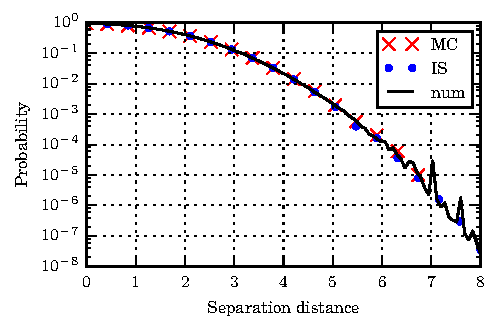
\includegraphics[width=\textwidth]{Images/Script_8_ISmc_1}
				%\caption{Probabilité estimé}
				\label{fig:ISmc}
			\end{minipage}
		\end{figure}}
		\only<3>{\begin{figure}[htbp]
			\centering
				\begin{minipage}[b]{0.9\textwidth}
					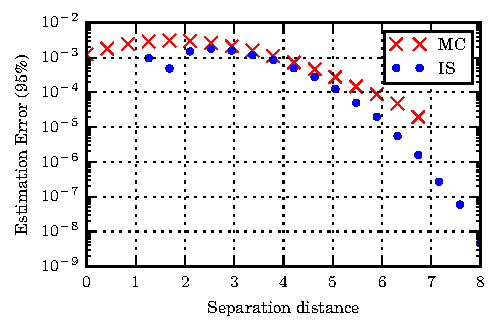
\includegraphics[width=\textwidth]{Images/Script_8_ISmc_2}
					%\caption{Erreur de les méthodes}
					\label{fig:ISmcErr}
				\end{minipage}
			%\caption{caption}
			\label{fig:label}
		\end{figure}}
		\only<4>{Calcul par méthode Constante}
		\only<4>{\begin{table}[htbp]
			\begin{center}
				\csvautobooktabular{Tables/ISconst.csv}
			\end{center}
			%\caption{Estimation avec IS type constant de la probabilité de collision}
			\label{tab:ISconst}
		\end{table}}
		\only<5>{Calcul par méthode Linéaire}
		\only<5>{\begin{table}[htbp]
			\begin{center}
				\csvautobooktabular{Tables/ISlin.csv}
			\end{center}
			%\caption{Estimation avec IS type linéaire de la probabilité de collision}
			\label{tab:ISlin}
		\end{table}}
		\only<6>{Calcul par méthode Toit}
		\only<6>{\begin{table}[htbp]
			\begin{center}
				\csvautobooktabular{Tables/IStoit.csv}
			\end{center}
			%\caption{Estimation avec IS type toit de la probabilité de collision}
			\label{tab:IStoit}
		\end{table}}
	\end{frame}
	%--- Next Frame ---%
	\begin{frame}[t]{Distribution conditionnée}
		Simulation à distance 4 avec un échantillon de $10^5$.
		\only<2>{\begin{figure}[htbp]
			\centering
			\begin{minipage}[b]{0.9\textwidth}
				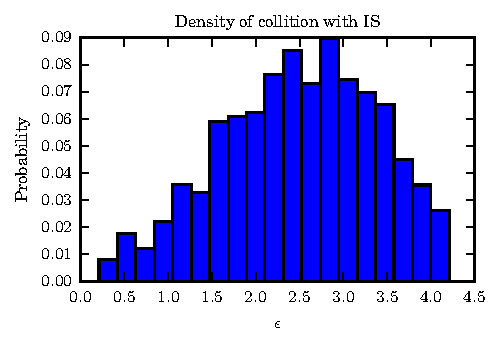
\includegraphics[width=\textwidth]{Images/Script_14_2}
				%\caption{Densité de probabilité obtenue avec IS}
				\label{fig:Dens1}
			\end{minipage}
			
		\end{figure}}
		\only<3>{\begin{figure}[htbp]
			\centering
				\begin{minipage}[b]{0.9\textwidth}
					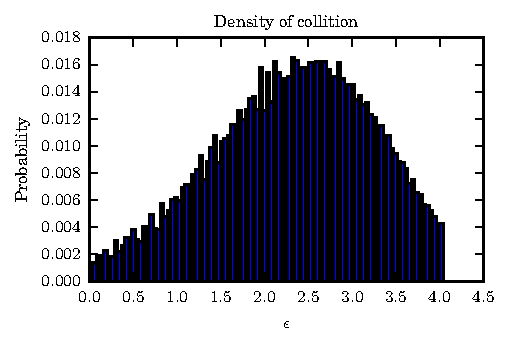
\includegraphics[width=\textwidth]{Images/Script_14_1}
					%\caption{Densité de probabilité obtenue numériquement}
					\label{fig:Dens2}
				\end{minipage}
			%\caption{caption}
			\label{fig:label}
		\end{figure}}
	\end{frame}
	%--- Next Frame ---%
	% subsection importance_sampling (end)

	\subsection{Méthode de Splitting} % (fold)
	\label{sub:methode_de_splitting}
	\begin{frame}[t]{Méthode de Splitting}
		On souhaite estimer $\mathbb{P}[\varphi(U)\leq \epsilon]$ avec $\varphi(U)$ le plus petit élément de $U$. On trouve une séquence $\epsilon_{k}>\ldots>\epsilon$ et on calcule 
			\begin{align*}
				\mathbb{P}[\varphi(U)\leq \epsilon] &= \mathbb{P}(\varphi(U)\leq \epsilon_{1}) \prod _{k=2}^{m} \mathbb{P}(\varphi(U)\leq \epsilon_{k}|\varphi(U)\leq \epsilon_{k-1})
			\end{align*}
			\begin{itemize}
				\item<2-> Avoir les probabilités dans un même ordre
				\item<3> Estimer les quantiles empiriques
			\end{itemize}
	\end{frame}
	%--- Next Frame ---%
	\begin{frame}[t]{Résultats}
		\only<1>{\begin{figure}[htbp]
			\centering
			\begin{minipage}[b]{0.9\textwidth}
				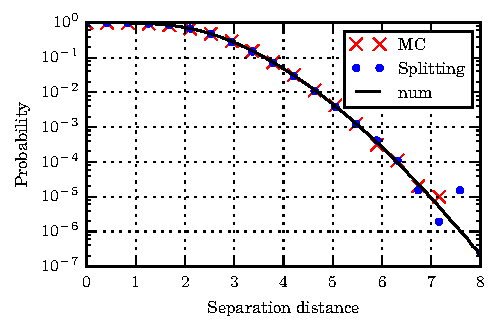
\includegraphics[width=\textwidth]{Images/Script_10_SplittingvsMC}
				%\caption{Probabilité estimé avec Splitting}
				\label{fig:Splitting}
			\end{minipage}
		\end{figure}}
		\only<2>{\begin{table}[htbp]
			\begin{center}
				\csvautobooktabular{Tables/Splitting.csv}
			\end{center}
			%\caption{Estimation avec Splitting de la probabilité de collision}
			\label{tab:Splitting}
		\end{table}}
	\end{frame}
	%--- Next Frame ---%
	% subsection methode_de_splitting (end)
	
	\subsection{Trajectoires Croisées} % (fold)
	\label{sub:trajectoires_croisees}
	
	\begin{frame}[t]{Trajectoires Croisées}
		Modélisation des trajectoires
		\only<1-3>{\begin{itemize}
			\item<+-> Rotation des trajectoires
			\item<+-> Prendre la différence entre elles $U=(U_x,U_y)$
			\item<+-> Estimer $\mathbb{P}(\sqrt{U_x^2 + U_y^2} < \epsilon)$
		\end{itemize}}
		\only<4>{\begin{figure}[htbp]
			\centering
			\begin{minipage}[b]{0.9\textwidth}
				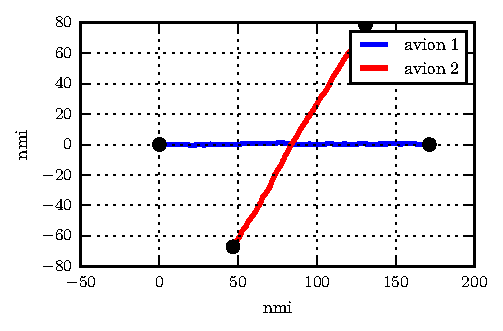
\includegraphics[width=\textwidth]{Images/Script_6_1}
				%\caption{Exemple de trajectoire}
				\label{fig:Croiss}
			\end{minipage}
		\end{figure}}
	\end{frame}
	%--- Next Frame ---%
	\begin{frame}[t]{Importance Sampling}
		Résultats
		\only<2>{\begin{table}[htbp]
			\begin{center}
				\csvautobooktabular{Tables/ISoblique.csv}
			\end{center}
			%\caption{Estimation avec IS de la probabilité de collision}
			\label{tab:Isobl}
		\end{table}}
	\end{frame}
	\begin{frame}[t]{Distribution Conditionnelle}
			\centering
			\only<1>{\begin{minipage}[b]{0.9\textwidth}
				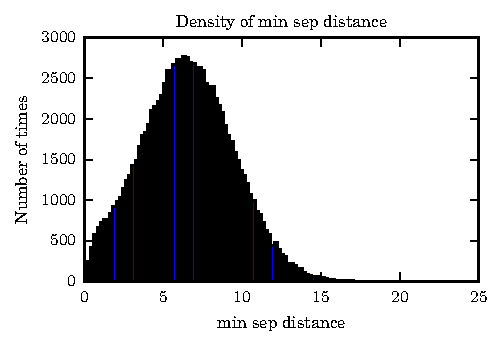
\includegraphics[width=\textwidth]{Images/Script_6_5}
				\label{fig:dist1}
			\end{minipage}}
			\only<2>{\begin{minipage}[b]{0.9\textwidth}
				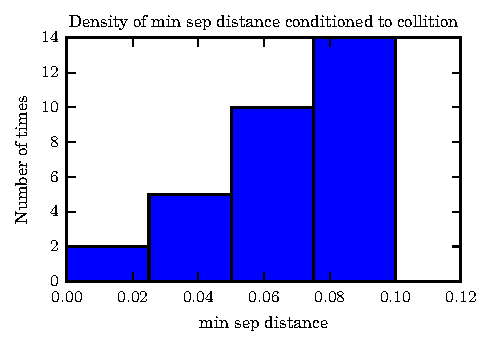
\includegraphics[width=\textwidth]{Images/Script_6_4}
				\label{fig:dist2}
			\end{minipage}}
	\end{frame}
	%--- Next Frame ---%
	% subsection trajectoires_croisees (end)
	% section resultats (end)
	
	\section{Conclusion} % (fold)
	\label{sec:conclusion}
	
	\begin{frame}[t]{Conclusion}
		\begin{itemize}
			\item<+-> Méthodes Implémentées
			\item<+-> Résultats obtenus
			\item<+-> Probabilité estimée
		\end{itemize}
	\end{frame}
	%--- Next Frame ---%
	\begin{frame}[c]{Fin}
		\begin{center}
		\Huge Merci
		\end{center}
	\end{frame}
	%--- Next Frame ---%
	% section conclusion (end)
\end{document}